\section{Introduction}
\label{sec:hybrid-intro}


Discovering relations among brain regions toward a specific phenotypic outcome from fMRI signals has been a crucial area in neuroimaging research. Reliable and informative relations help neuroscientists and clinical professionals to better understand brain functions, and thus improve clinical diagnosis and treatments \citep{kucian2008development,kucian2006impaired, li2015putting,li2015toward,satterthwaite2015linked,wang2016efficient}.
However, despite the clear multiplexity of the brain's involvement in cognition \citep{logue2014neural,barrasso2016neurobiological,knauff2010complex,reineberg2022context}, current imaging biomarker detection methods \citep{shen2017using,gao2019combining,li2021braingnn} focus only on the contributing roles of the pairwise connectivity edges. In contrast, most brain functions involve distributed patterns of interactions among multiple regions \citep{semedo2019cortical}. For instance, executive planning requires the appropriate communication of signals across many distinct cortical areas \citep{logue2014neural}. 
These high-order relationships, cannot always be decomposed into pairwise ones \cite{battiston2020networks, battiston2021physics, bick2023higher}, thus allowing them to capture information beyond the reach of pairwise ones \cite{do2020structural}. Consequently, relying solely on pairwise connectivity, without accounting for the brain's complex high-order structure, may result in inconsistent findings and low predictive performance across studies. 
Although recently there have been a few works \citep{zu2016identifying,xiao2019multi,li2022construction} working on discovering the high-order relationships of brain regions, they are unable to effectively extract meaningful patterns. This is because these methods usually first identify some candidates of high-order relationships and then perform feature selection. The candidates are obtained by enumerating only a small portion of all possible relations, or by clustering methods that are unrelated to the target. As a result, most informative high-order relations are likely excluded at the first stage. This inspires us to solve the problem in an end-to-end manner through a more expressive model and a more appropriate objective.

%1) the discovering process of high-order relationships is not guided by cognitive targets; 2) the weak expressiveness of traditional machine learning methods (e.g. lasso regression) hinders the accurate modeling of brain region interactions \citep{cao2022brain,richards2019deep}.

In this paper, we aim to identify high-order relationships that are informative towards a phenotypic outcome, such as a cognition score. However, unlike pairwise relations, the number of possible high-order relations is exponential. To identify the most informative ones from the exponential space, we propose our objective: \textit{maximally informative and minimally redundant} (MIMR). That is to say, we maximize the information contained in the high-order relationships towards a neurological outcome (\textit{informativeness}) while diminishing the participation of unrelated brain regions (\textit{redundant}).
% \todo{more citations in this paragraph to justify the principle would be awesome. We could even move some of the citations from previous paragraphs here if relevant.} 
Such a criterion, on the one hand, ensures the predictive performance of these high-order relationships; on the other hand, it endows the model with the capacity to identify more succinct and interpretable structures \citep{yu2020graph,miao2022interpretable,miao2022interpretable2,chen2023tempme}. A formal definition of the MIMR criterion could be found in Equation \ref{equ:ib2} from an information bottleneck point of view.

\begin{figure}
    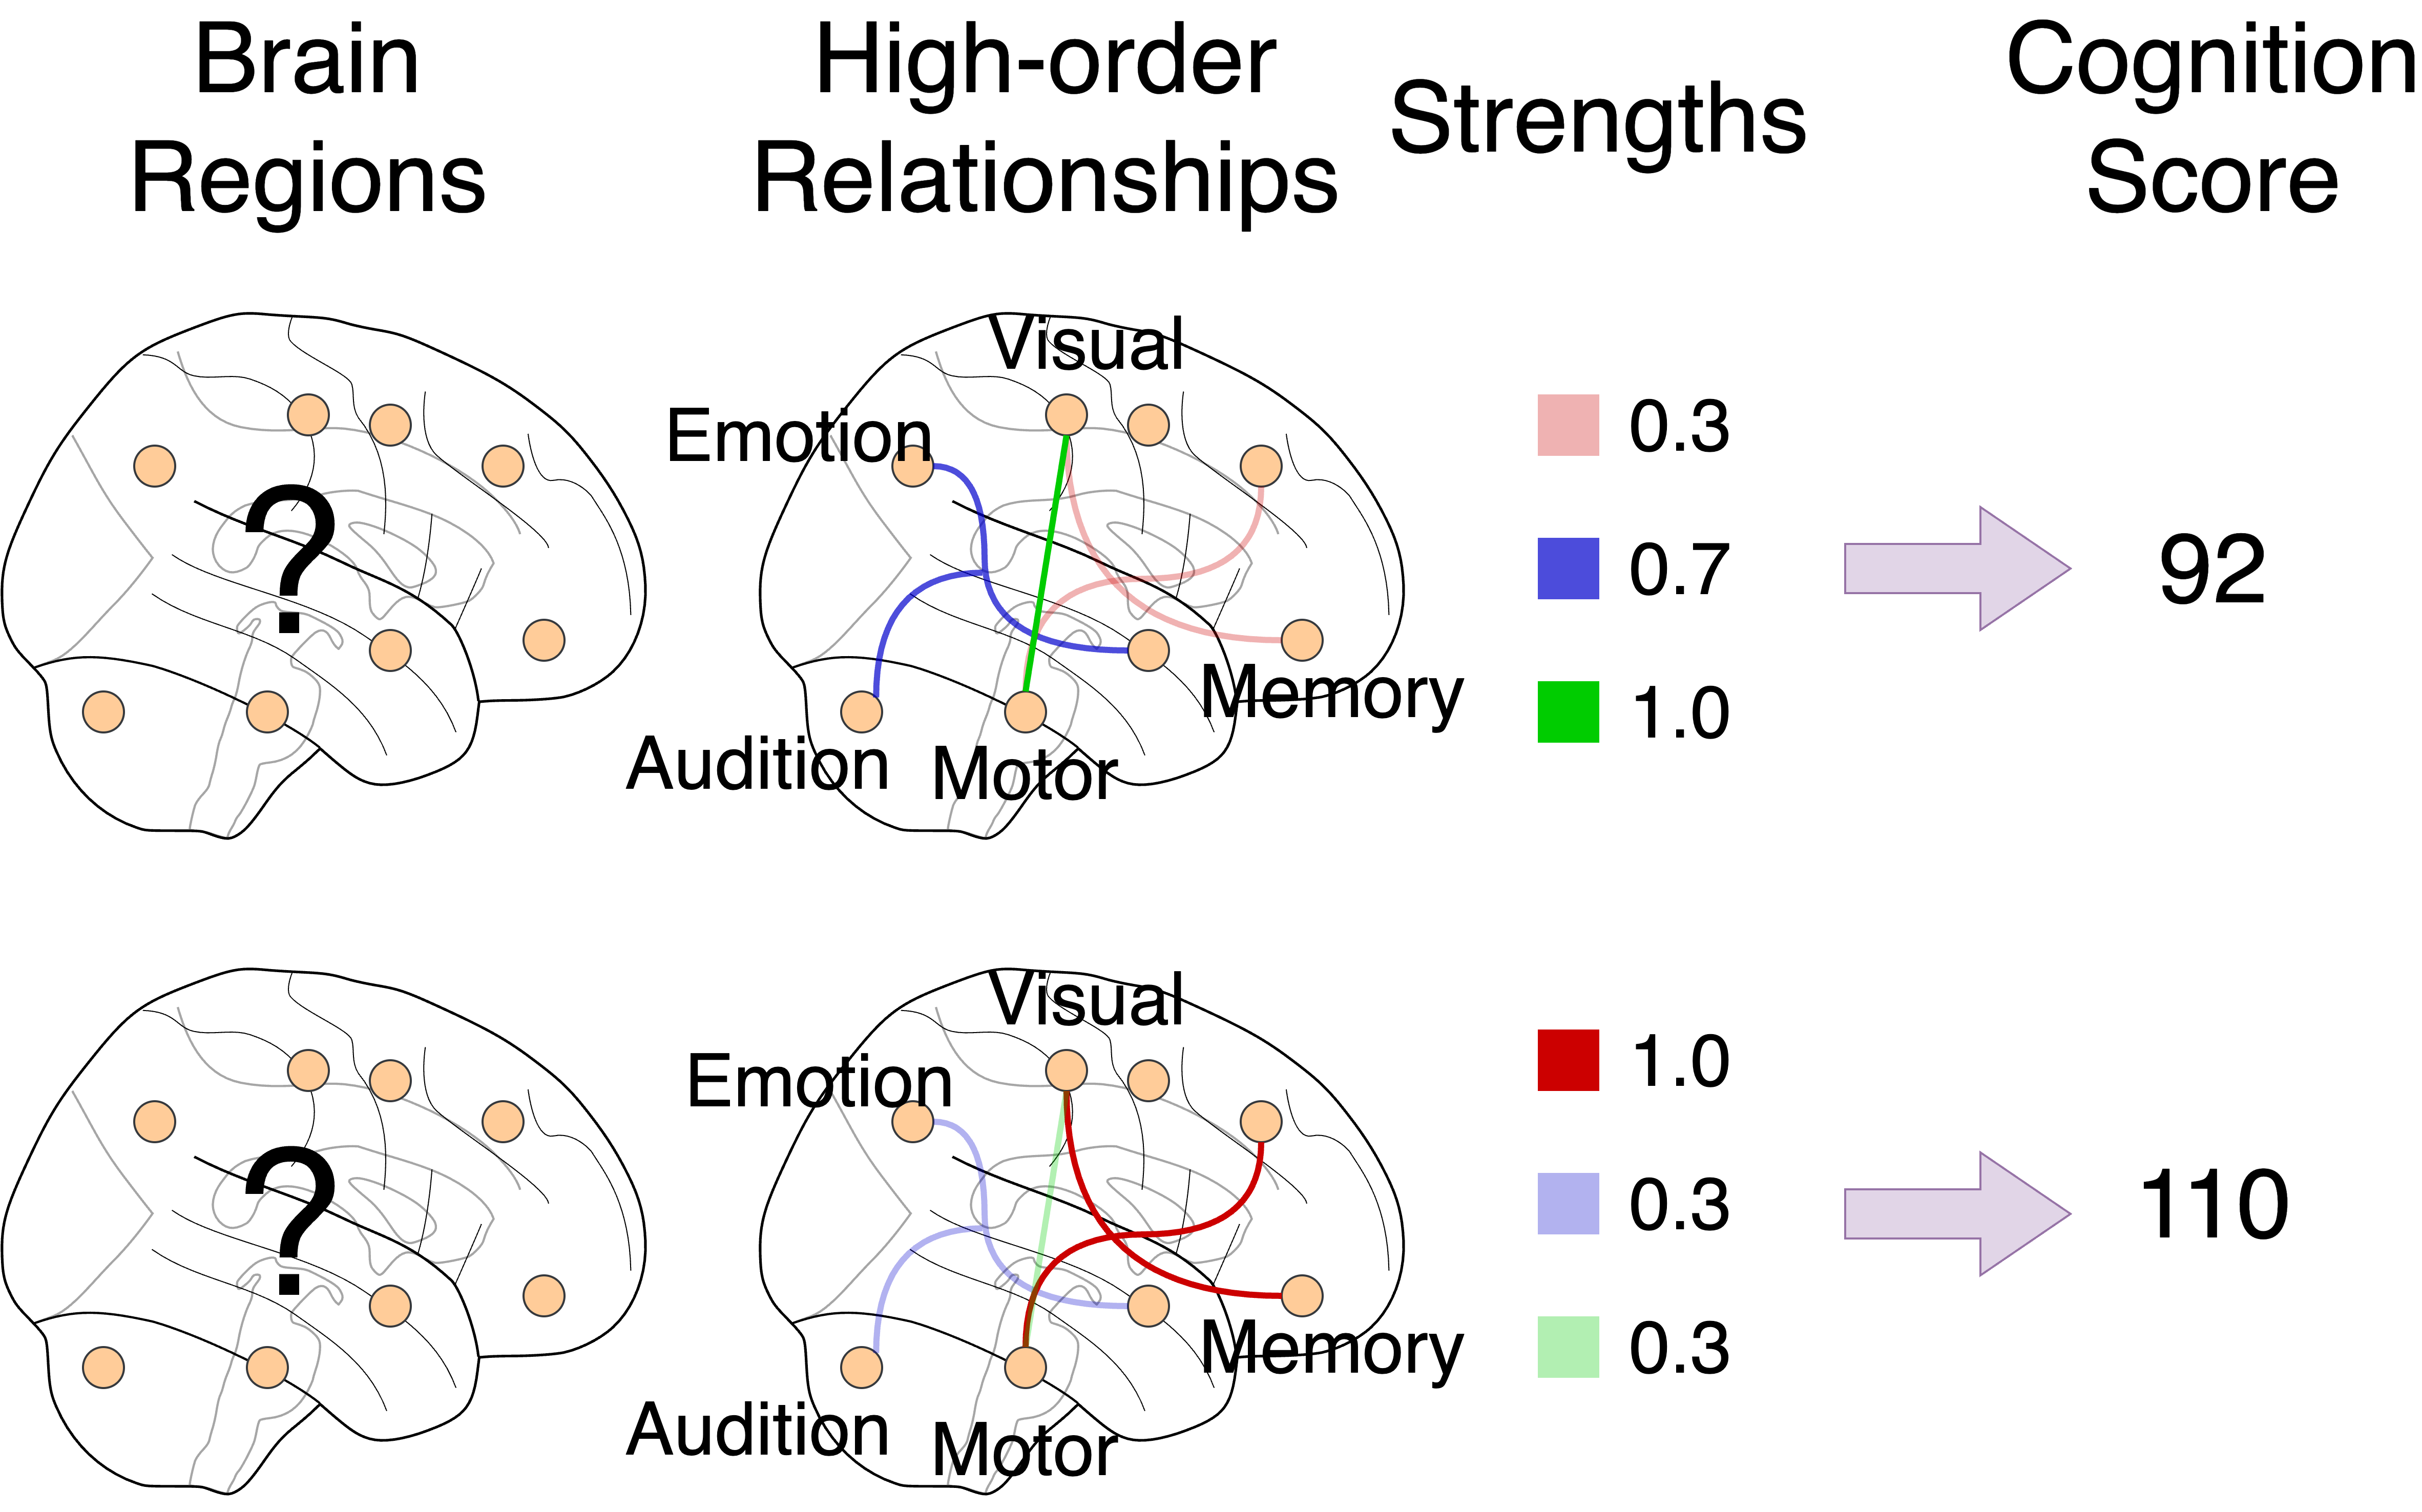
\includegraphics[width=\linewidth]{figures/tasting400.png}
    % \vskip 0.1in
    \caption{We identify high-order relationships of brain regions, where hyperedge structures and weights possess strong relevance to cognition (maximal informativeness). Meanwhile, they contain the least irrelevant information.}
    \label{fig:tasting}
% \vskip -0.1in
    
\end{figure}

% This property, on the one hand, ensures the high-order relationships encapsulate sufficient information related to cognition, which prevents the omission of any of them that makes a significant contribution to cognition. On the other hand, it allows us to diminish irrelevant ones, which will make the results as succinct as possible.


% \htl{we (propose to) formulate the capture of high-order relationship in the brain as the construction of the hypergraph, where the nodes are regions and the hyperedges connect all the related regions.}
% \htl{To better...(require a motivation of why MRMI), a desired hypergraph should maximize the correlation between hyperedges and the predicted property while diminishing the correlation with unrelated inputs, which is also demonstrated by xxx.}

% \htl{However, most of the previous works on hypergraph construction fail to xxx since }

We formulate high-order relationships as weighted hyperedges in a hypergraph, where regions are treated as nodes. Unlike a traditional graph where edges connect only two nodes, a hypergraph allows edges, known as hyperedges, to connect any number of nodes. The hypergraph should be weighted, and the weights of hyperedges are considered as strengths of high-order relationships, which contain the information relevant to the outcome (Figure \ref{fig:tasting}). 
% Therefore, our goal is to construct a weighted hypergraph model of each brain, where the nodes are regions and hyperedges are set to be identified. These hyperedges should be maximally informative and minimally redundant: \textit{informativeness} is the mutual information between the hyperedges and the prediction target (e.g. cognition score).
% We maximize it because we expect these hyperedges to carry more information about the target; \textit{redundancy} is the mutual information between the hyperedges and the inputs. We minimize it because we expect succinct relations. Acquiring such maximally informative and minimally redundant hyperedges is much more challenging than pairwise edges in a normal graph due to the exponential search space since the number of nodes connected by a hyperedge can be arbitrary.\htl{better to separate it into two sentences "...due to...since"}

% In addition, \stodo{perhaps ad
% isk of overfitting in the model.

However, current methods for hypergraph construction, which are mostly based on neighbor distances and neighbor reconstruction \citep{wang2015visual,liu2017elastic,jin2019robust,huang2009video}, are unsuitable in our context for several reasons: 1) they are unable to learn MIMR hyperedges due to the absence of a tractable objective for learning such hyperedges.  2) they fall short of learning consistent structures across subjects, which contradicts the belief that the cognitive function mechanism of healthy human beings should be similar \citep{wang2023inference}. 3) the number of hyperedges is restricted to the number of nodes, which may lead to sub-optimal performance. Furthermore, although information bottleneck (IB) has been a prevailing solution to learn MIMR representations in deep learning \citep{kim2021drop,alemi2016deep,luo2019significance}, existing IB methods focus on extracting compressed representations of inputs instead of identifying underlying structures such as hypergraphs. Harnessing the IB framework for identifying hypergraphs necessitates both architectural innovations and theoretical derivations.

\paragraph{Proposed Work} In this paper, we propose \textbf{Hy}pergraph of \textbf{B}rain \textbf{R}egions via mult\textbf{i}-head \textbf{D}rop-bottleneck (\mname{}), a novel approach for identifying maximally informative yet minimally redundant high-order relationships of brain regions. The overall pipeline of \mname{} is depicted in Figure \ref{fig:pipeline}. \mname{} is equipped with a \textsc{Constructor} and a \textsc{Weighter}. The \textsc{Constructor} identifies the hyperedge structures of brain regions by learning sets of masks, and the \textsc{Weighter} computes a weight for each hyperedge. To advance the IB principle for hyperedge identification, we further propose \textit{multi-head drop-bottleneck} and derive its optimization objective.

\mname{} avoids searching in an exponential space through learning masks to identify hyperedges, which guarantees efficiency. Its feature-agnostic masking mechanism design ensures \mname{} to learn consistent structures across subjects. Moreover, the model is equipped with a number of parallel heads, each of which is dedicated to a hyperedge. Through this, \mname{} is able to identify any number of hyperedges, depending on how many heads it is equipped with. Additionally, the proposed \multiheadname{} theoretically guarantees the maximal informativeness and minimal redundancy of the identified hyperedges. 

% To alleviate the data scarcity issue, \mname{} is equipped with a special architecture, where some components are shared by all datasets, and others are specific to the condition.

We evaluate our methods on the open-source ABIDE dataset and the restricted ABCD dataset. We quantitatively evaluate our approach by a commonly used protocol for studying brain connections, CPM~\citep{shen2017using} (Appendix \ref{sec:app_cpm}), and show that our model outperforms the state-of-the-art deep learning models by an average of $11.2\%$ on a comprehensive benchmark. Our post-hoc analysis demonstrates that hyperedges of higher degrees are considered more significant, which indicates the significance of high-order relationships in human brains.